\documentclass{standalone}
\usepackage{graphicx}	
\usepackage{amssymb, amsmath, amsthm}
\usepackage{color}

\usepackage{tikz}
\usetikzlibrary{intersections, backgrounds, arrows.meta}

\definecolor{light}{RGB}{220, 188, 188}
\definecolor{mid}{RGB}{185, 124, 124}
\definecolor{dark}{RGB}{143, 39, 39}
\definecolor{highlight}{RGB}{180, 31, 180}
\definecolor{gray10}{gray}{0.1}
\definecolor{gray20}{gray}{0.2}
\definecolor{gray30}{gray}{0.3}
\definecolor{gray40}{gray}{0.4}
\definecolor{gray60}{gray}{0.6}
\definecolor{gray70}{gray}{0.7}
\definecolor{gray80}{gray}{0.8}
\definecolor{gray90}{gray}{0.9}
\definecolor{gray95}{gray}{0.95}

\begin{document}

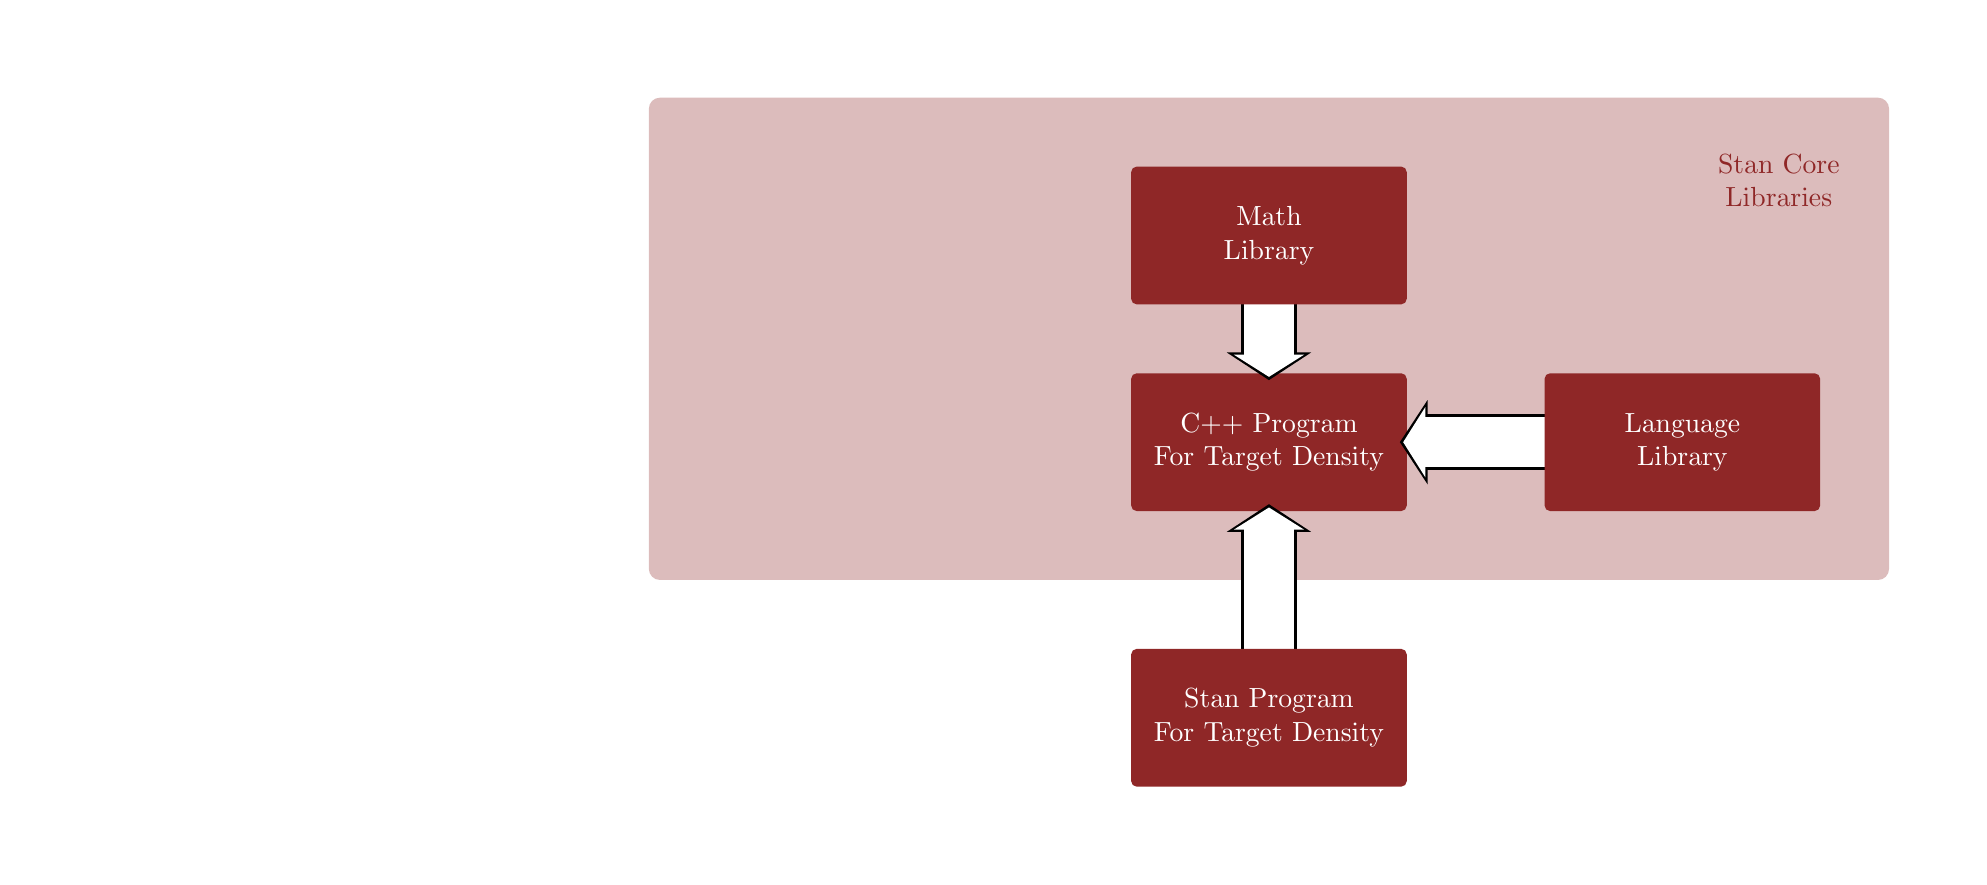
\begin{tikzpicture}[scale=0.35, thick]
  \draw[white] (-37.5, -12.5) rectangle (32.5, 17.5);
  
  \fill[rounded corners=4pt, light] (-15, -2.5) rectangle +(45, 17.5);
  \node[text=dark, align=center] at (26, 12) { Stan Core\\Libraries };
  
  \fill [rounded corners=2pt, fill=dark, text=white] (2.5, 0) rectangle +(10, 5) 
  node[midway, align=center] { C++ Program\\For Target Density };

  \draw[line width=20, -{Triangle[width=30,length=10]}] (17.5, 2.5) -- +(-5.25, 0);
  \draw[line width=18, -{Triangle[width=25,length=8]}, white] (17.5, 2.5) -- +(-5.13, 0);

  \fill [rounded corners=2pt, fill=dark, text=white] (17.5, 0) rectangle +(10, 5) 
  node[midway, align=center] { Language\\Library };

  \draw[line width=20, -{Triangle[width=30,length=10]}] (7.5, -5) -- +(0, 5.25);
  \draw[line width=18, -{Triangle[width=25,length=8]}, white] (7.5, -5) -- +(0, 5.13);
  
  \fill [rounded corners=2pt, fill=dark, text=white] (2.5, -10) rectangle +(10, 5) 
  node[midway, align=center] { Stan Program\\For Target Density };

  \draw[line width=20, -{Triangle[width=30,length=10]}] (7.5, 7.5) -- +(0, -2.75);
  \draw[line width=18, -{Triangle[width=25,length=8]}, white] (7.5, 7.5) -- +(0, -2.63);

  \fill [rounded corners=2pt, fill=dark, text=white] (2.5, 7.5) rectangle +(10, 5) 
  node[midway, align=center] { Math\\Library };
  
\end{tikzpicture}

\end{document}  